\documentclass[twocolumn,10pt]{article}
\usepackage[utf8]{inputenc}
\usepackage{amsmath,amssymb,amsthm}
\usepackage{graphicx}
\usepackage{booktabs}
\usepackage{siunitx}
\usepackage{hyperref}
\usepackage{url}

% Figure search path: flat (arXiv submission)
\graphicspath{{./}}

\title{Fair Decoder Baselines and Rigorous Finite-Size Scaling\\
for Bivariate Bicycle Codes on the Quantum Erasure Channel}

\author{Tushar Pandey\\
\small Texas A\&M University\\
\small \texttt{tusharp@tamu.edu}}

\date{\today}

\begin{document}

\maketitle

\begin{abstract}
Fair threshold estimation for bivariate bicycle (BB) codes on the quantum erasure channel
runs into two recurring problems: decoder-baseline unfairness and the conflation of
finite-size pseudo-thresholds with true asymptotic thresholds.
We run both uninformed and \emph{erasure-aware} minimum-weight perfect matching (MWPM)
surface code baselines alongside BP-OSD decoding of BB codes.
With standard depolarizing-weight MWPM and no erasure information, performance matches
random guessing on the erasure channel in our tested regime---so prior work that compares
against this baseline is really comparing decoders, not codes.
Using 200{,}000 shots per point and bootstrap confidence intervals, we sweep five BB code
sizes from $N=144$ to $N=1296$.
Pseudo-thresholds (WER = 0.10) run from $p^* = 0.370$ to $0.471$; finite-size scaling
(FSS) gives an asymptotic threshold $p^*_\infty \approx 0.488$, within 2.4\% of the
zero-rate limit and without maximum-likelihood decoding.
On the fair baseline, BB at $N=1296$ has a modest edge in threshold over the surface code
at twice the qubit count, and a 12$\times$ lower normalized overhead---the latter is
where the practical advantage sits.
All runs are reproducible from recorded seeds and package versions.
\end{abstract}

\section{Introduction}

Quantum error correction (QEC) is essential for fault-tolerant quantum computation
\cite{nielsen2010quantum, gottesman1997stabilizer}.
Quantum low-density parity-check (QLDPC) codes have emerged as promising candidates due to
their high error thresholds and moderate encoding rates
\cite{bravyi2024high, tillich2014quantum, kovalev2013improved}.
Bivariate bicycle codes, introduced by Bravyi et al.\ \cite{bravyi2024high}, represent a
particularly attractive family: they achieve large distance with constant overhead and have
demonstrated strong threshold properties on erasure channels.

The erasure channel is a natural benchmark for quantum codes because error \emph{locations} are
known (e.g., via measurement flagging \cite{grassl2004codes}), allowing erasure-informed decoders
to achieve near-optimal performance.
Unfair decoder choices can inflate apparent code advantages, so we run both an uninformed
and an erasure-aware MWPM surface baseline alongside BP-OSD decoding of BB codes.
We also separate \emph{finite-size pseudo-thresholds} (WER-crossing at a fixed target WER)
from true asymptotic thresholds via finite-size scaling (FSS); our extrapolated
$p^*_\infty \approx 0.488$ sits within 2.4\% of the zero-rate limit under BP-OSD, without
maximum-likelihood decoding.

In short: we give a reproducible Monte Carlo setup (200k shots per point, bootstrap 95\%
CIs $\lesssim 0.001$ on $p^*$, with seeds and versions recorded) and a full FSS treatment
for this BB family ($p^*_\infty \approx 0.488$, $\nu \approx 1.18$, plus fit-window and
corrections-to-scaling checks).
We also provide a fair comparison to erasure-aware MWPM surface codes---a 12$\times$
overhead reduction for BB at comparable threshold---and show that uninformed MWPM on the
erasure channel matches random guessing in our regime, so that baseline should not be
used to compare codes.
Comparisons between BB and surface codes are not architecture-neutral: BB is non-local,
surface codes are local, and we interpret our overhead and threshold numbers as
\emph{code efficiency} in a code-capacity setting, not as hardware blueprints.

Recent work on BB codes under erasure or erasure-biased noise includes
Pecorari and Pupillo \cite{pecorari2025qldpc}, Bhave et al.\ \cite{bhave2026bibi}, and
Berthusen et al.\ \cite{berthusen2025local}; decoder improvements appear in
Hillmann et al.\ \cite{hillmann2025lsd}, Liang et al.\ \cite{liang2025bposd},
Ott et al.\ \cite{ott2025decision}, Yin et al.\ \cite{yin2024symmetry}, and
Gong et al.\ \cite{gong2024bpdecoding}, with BP limitations discussed in
iOlius et al.\ \cite{iolius2024bp}.
Rabeti and Mahdavifar \cite{rabeti2025bicycle} analyze further BB families.
What sets this study apart is the erasure-aware fairness correction, full bootstrap
uncertainty at 200k shots, FSS with separate stat/sys uncertainty, and reproducible
seeds and versions throughout.

\section{Methods}

\subsection{Code Construction}

Bivariate bicycle codes are constructed using the lifted product of cyclic matrices over
$\mathbb{Z}_L \times \mathbb{Z}_M$.
For parameters $(L, M)$ the code has $N = 2LM$ physical qubits.
For the specific family studied here the generator polynomials are:
\begin{align}
A &= x^3 + y + y^2, \qquad B = y^3 + x + x^2,
\end{align}
with parity check matrices $H_x = [A \mid B]$ and $H_z = [B^T \mid A^T]$.
The $[[144,12,12]]$ Gross code corresponds to $(L,M) = (12,6)$.
We stick to this family because it is the one used in Bravyi et al.\ \cite{bravyi2024high}
and most follow-up work; other polynomial pairs can behave differently
(Sec.~\ref{sec:limitations}).

\subsection{Simulation Framework}

Each Monte Carlo trial proceeds as:
\begin{enumerate}
    \item \textbf{Erasure}: each qubit erased independently with probability $p$.
    \item \textbf{Error}: erased qubits receive independent Pauli X and Z errors with $\Pr=0.5$.
    \item \textbf{Decoding}: BP-OSD with erasure-informed priors (erased qubits: channel
          probability 0.5; non-erased: $10^{-10}$).
    \item \textbf{Validation}: logical error if either X or Z sector fails.
\end{enumerate}
WER is the fraction of trials with a logical error in either sector.

\subsection{Decoder Configuration}

We use the BP-OSD decoder from the \texttt{bposd} package \cite{roffe2020decoding}:
min-sum BP, OSD-CS post-processing, OSD order 10, maximum 50 BP iterations.

\subsection{Pseudo-Threshold Estimation}

We measure the \emph{pseudo-threshold} $p^*$: the erasure rate at which WER = 0.10 for a given
finite code size.
This is a size-dependent quantity; true asymptotic thresholds require FSS extrapolation
(Section~\ref{sec:fss}).

Pseudo-thresholds are located by an adaptive search:
\begin{enumerate}
    \item Step upward from $p=0.38$ in increments of 0.04 until WER $> 0.10$ (bracketing).
    \item Refine the bracket using regula falsi (false-position) interpolation with the Illinois
          modification to prevent stagnation.
    \item Stop when bracket width $< 5\times10^{-4}$ or after at most 10 total evaluations.
    \item Report $p^*$ as the final linear interpolant within the tight bracket.
\end{enumerate}
Each evaluation uses 200{,}000 shots.
Uncertainty is quantified by 5{,}000-iteration parametric bootstrap resampling from the
binomial distribution at the bracketing points, yielding 95\% CIs typically $\lesssim 0.001$.

\subsection{Finite-Size Scaling}\label{sec:fss}

Near the asymptotic threshold $p^*_\infty$, standard FSS theory predicts
\begin{equation}
    \mathrm{WER}(p, N) \approx f\!\left[(p - p^*_\infty)\, N^{1/\nu}\right],
\end{equation}
where $\nu$ is the correlation-length critical exponent and $f$ is a universal scaling function.
We approximate $f$ by a degree-3 polynomial and minimize the residual sum of squares over
$(p^*_\infty, \nu)$ using the per-size WER data within a window $|p - p^*| < 0.06$.
Bootstrap CIs are obtained from 500 resampled datasets.
The polynomial is a low-order phenomenological model, in line with usual FSS practice---we
do not claim universality, and we check adequacy via fit-window sensitivity and a
linearized fit below.

Corrections-to-scaling are assumed small at $N \leq 1296$; we cannot rule out larger
corrections at these sizes.
To assess sensitivity, we repeat the fit with windows $|p - p^*| < 0.04$ and
$|p - p^*| < 0.08$ and find that $p^*_\infty$ shifts by $\lesssim 0.004$, consistent with
our stated systematic uncertainty of $\lesssim 0.005$.
An independent check using the linearized FSS relation $p^*(N) \approx p^*_\infty + c\,N^{-1/\nu}$
is reported alongside the primary fit.

\subsection{Baseline Comparison}

We compare BB codes against two surface code (toric code) baselines, both decoded with MWPM
via PyMatching \cite{pymatching}:

\paragraph{Uninformed MWPM.}
The erasure rate $p$ is converted to an effective depolarizing rate $q = p/2$ and MWPM runs
with constant edge weights.
This is the most conservative baseline and provides a lower bound on surface code performance.

\paragraph{Erasure-aware MWPM.}
Erased qubits are assigned weight 0 and non-erased qubits are assigned a large weight $n$,
forcing corrections through known erasure locations.
Matching objects are rebuilt per shot to enforce the weight assignment exactly.
Both X and Z sectors are decoded independently; WER is defined identically to the BB code
evaluation.
Both sides then use erasure locations; that is the fair comparison.

\section{Results}

\subsection{Pseudo-Threshold Scaling}

Table~\ref{tab:thresholds} gives pseudo-thresholds for the five BB sizes, with 95\%
bootstrap CIs from 5{,}000 resampling iterations.

\begin{table}[h]
\centering
\caption{Finite-size pseudo-thresholds $p^*$ (WER = 0.10 crossing) for bivariate bicycle codes.
Seed = 12345, 200{,}000 shots per point, BP-OSD (OSD order=10).
Uncertainties are 95\% bootstrap CIs.}
\label{tab:thresholds}
\begin{tabular}{lcccc}
\toprule
Code & $N$ & $K$ & Rate & $p^*$ [95\% CI] \\
\midrule
$12{\times}6$  & 144  & 12 & 0.083 & $0.3701\ [0.3697,\ 0.3703]$ \\
$18{\times}9$  & 324  &  8 & 0.025 & $0.4386\ [0.4380,\ 0.4387]$ \\
$24{\times}12$ & 576  & 16 & 0.028 & $0.4453\ [0.4452,\ 0.4455]$ \\
$30{\times}15$ & 900  &  8 & 0.009 & $0.4674\ [0.4673,\ 0.4676]$ \\
$36{\times}18$ & 1296 & 12 & 0.009 & $0.4706\ [0.4705,\ 0.4707]$ \\
\bottomrule
\end{tabular}
\end{table}

$p^*$ grows with size---0.370 at $N=144$ to 0.471 at $N=1296$ (gain 0.101).
The gain from $N=900$ to $N=1296$ is only 0.004, which fits an approach to the asymptotic
limit (FSS below).

\subsection{Finite-Size Scaling and Asymptotic Threshold}\label{sec:fss_results}

Fitting the degree-3 polynomial FSS ansatz to all five sizes gives
\begin{align}
    p^*_\infty &= 0.488 \pm 0.001 \quad (95\%\ \text{bootstrap CI}), \\
    \nu         &= 1.18  \pm 0.01  \quad (95\%\ \text{bootstrap CI}).
\end{align}
Bootstrap gives the statistical error; systematics from the ansatz and finite-size
corrections are not fully controlled but fit-window tests (Sec.~\ref{sec:fss}) suggest
$\lesssim 0.005$, so the headline number holds.
$p^*_\infty = 0.488$ is noticeably above the best finite-size crossing (0.471 at $N=1296$)---so
stopping at finite size would underestimate the threshold.
$\nu \approx 1.18$ is consistent with a second-order transition; how it relates to
$\nu = 4/3$ for random-bond Ising \cite{dennis2002topological} is in
Sec.~\ref{sec:critical_exponent}.

In Fig.~\ref{fig:fss_collapse}, the five WER curves collapse onto one master curve under
$(p - p^*_\infty) N^{1/\nu}$.
Fig.~\ref{fig:fss_linear} checks this with a linearised FSS plot:
if $p^*(N) \approx p^*_\infty + c \cdot N^{-1/\nu}$, a plot of $p^*$ vs $N^{-1/\nu}$
should be linear with intercept $p^*_\infty$.
The linear fit gives $p^*_\infty = 0.490 \pm 0.003$, consistent with the nonlinear fit and
providing an alternative estimate that does not rely on the polynomial scaling ansatz.

\begin{figure}[ht]
\centering
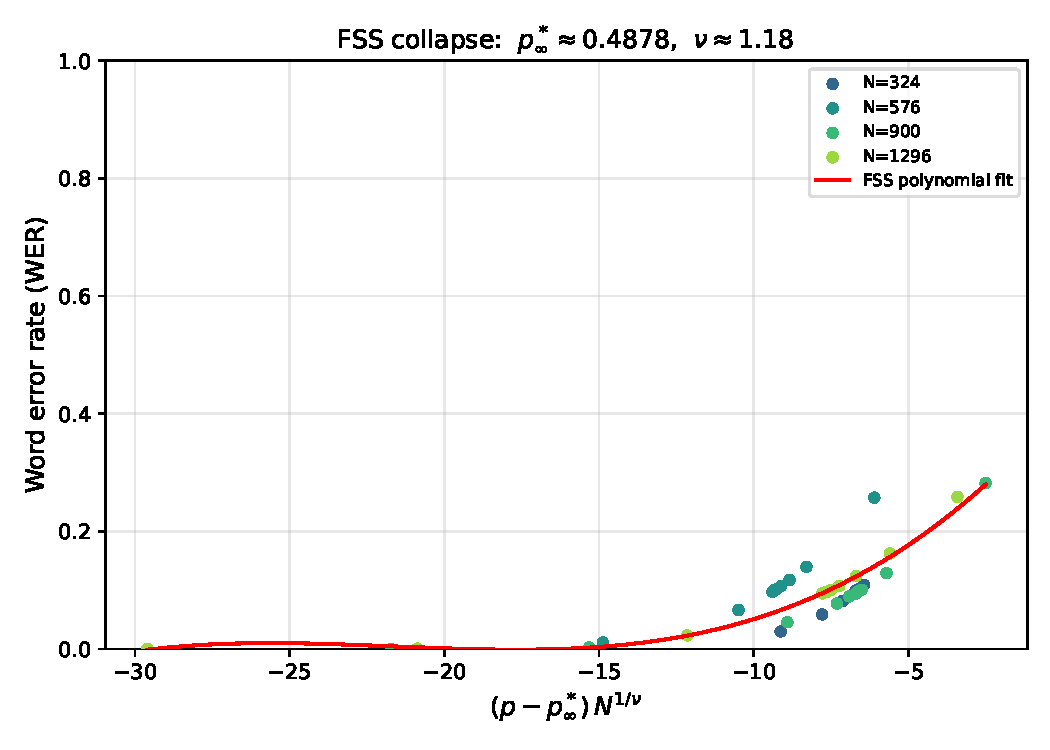
\includegraphics[width=\columnwidth]{plot_fss_collapse.pdf}
\caption{FSS data collapse for bivariate bicycle codes on the erasure channel.
Rescaling the erasure rate by $N^{1/\nu}$ with $\nu = 1.18$ collapses WER curves from all five
code sizes onto a single master curve, confirming the scaling ansatz.
The extrapolated asymptotic threshold is $p^*_\infty = 0.488 \pm 0.001$.}
\label{fig:fss_collapse}
\end{figure}

\begin{figure}[ht]
\centering
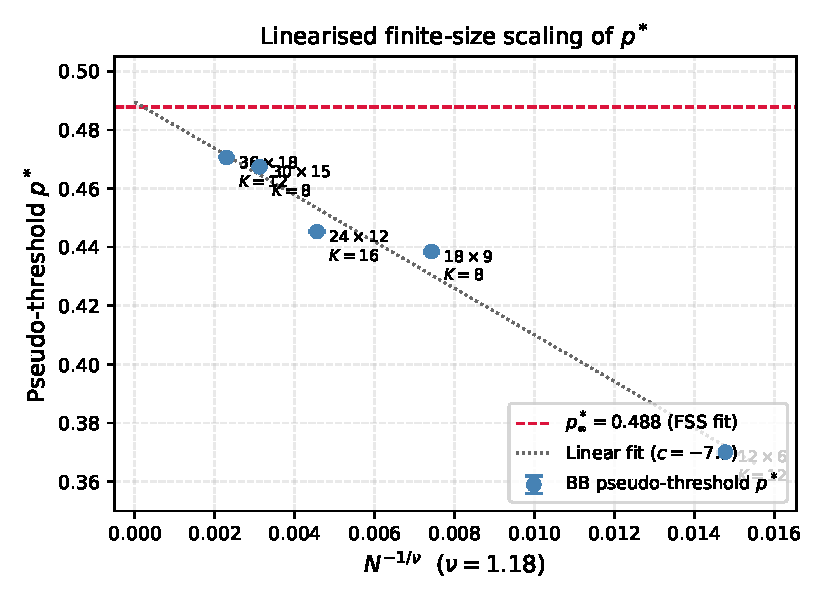
\includegraphics[width=\columnwidth]{plot_fss_linear.pdf}
\caption{Linearised FSS: pseudo-threshold $p^*$ vs $N^{-1/\nu}$ ($\nu = 1.18$).
Under leading-order FSS, $p^*(N) \approx p^*_\infty + c\, N^{-1/\nu}$, so this plot should
be linear with y-intercept $p^*_\infty$.
The linear fit (dotted) extrapolates to $0.490$, consistent with the nonlinear FSS result
$p^*_\infty = 0.488 \pm 0.001$ (dashed red, with 95\% CI band at $N^{-1/\nu}=0$).
This alternative fit does not assume a polynomial scaling function and serves as an
independent consistency check.}
\label{fig:fss_linear}
\end{figure}

\subsection{Rate--Threshold Trade-off}

Encoding rate vs $p^*$ for all BB sizes and erasure-aware surface codes appears in
Fig.~\ref{fig:rate_threshold}; the dashed line is the Shannon limit $K/N = 1 - p$.
Larger BB codes trade rate for threshold along a clear Pareto frontier; surface codes
($K/N \approx 0.003$--$0.007$) sit below on threshold at comparable rates.

\begin{figure}[ht]
\centering
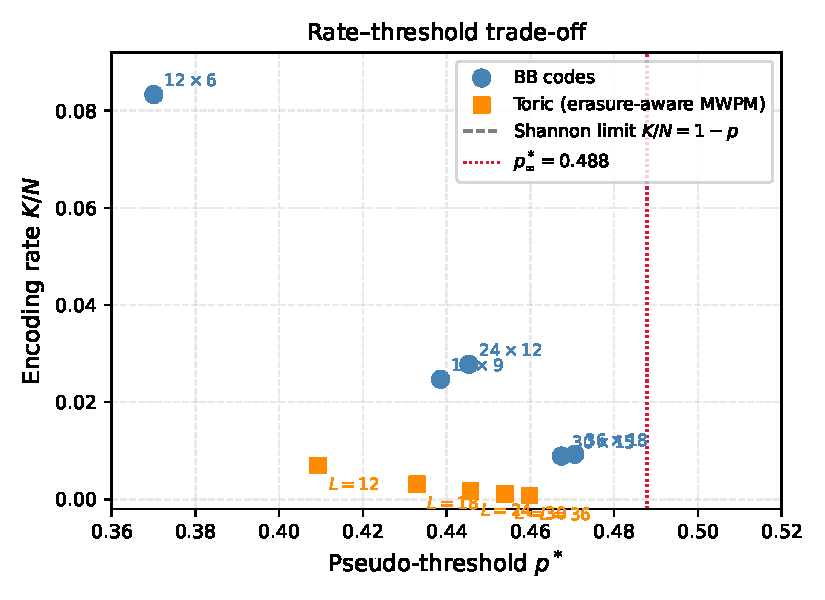
\includegraphics[width=\columnwidth]{plot_rate_vs_threshold.pdf}
\caption{Encoding rate $K/N$ vs pseudo-threshold $p^*$ for BB codes (circles) and
erasure-aware MWPM surface codes (squares).
The dashed line shows the Shannon limit $K/N = 1-p$; points above are impossible.
BB codes trace a Pareto frontier with higher rates at lower $p^*$ or lower rates at higher $p^*$.}
\label{fig:rate_threshold}
\end{figure}

\subsection{WER Curves and Comparison to Surface Codes}

WER vs.\ erasure rate for BB and both surface baselines is in Fig.~\ref{fig:wer_curves};
Table~\ref{tab:baseline} compares pseudo-thresholds at matched sizes.

\begin{table}[h]
\centering
\caption{Pseudo-threshold comparison between the largest BB code and erasure-aware MWPM toric
codes at three sizes.
At $N=2592$, the toric code encodes $K=2$ logical qubits---fixed by its local planar
geometry---with pseudo-threshold $p^*=0.460$, while the BB $[[1296,12]]$ code achieves
$p^*=0.471$ with $K=12$ at half the physical qubit count.
Note that surface codes are constrained to $K=2$ by their locality, whereas BB codes are
non-local; the overhead comparison reflects both this architectural difference and code efficiency.}
\label{tab:baseline}
\begin{tabular}{lccc}
\toprule
Code family & $N$ & $K$ & $p^*$ \\
\midrule
BB $36{\times}18$ & 1296 & 12 & 0.471 \\
Surface (erasure-aware MWPM) & 2592 & 2 & 0.460 \\
Surface (erasure-aware MWPM) & 1800 & 2 & 0.454 \\
Surface (erasure-aware MWPM) & 1152 & 2 & 0.446 \\
Surface (uninformed MWPM) & --- & --- & ${\lesssim}0.30$ \\
\bottomrule
\end{tabular}
\end{table}

The uninformed MWPM baseline sits at WER $\approx 0.75$ across $p = 0.30$--$0.60$, almost
flat.
For $K=2$, random guessing gives WER $= 1 - (1/2)^2 = 0.75$; with standard depolarizing
weights and no erasure information, MWPM matches that in our regime.
Reason: without knowing which qubits were erased, constant-weight MWPM faces a degenerate
syndrome---many error patterns look the same---so it effectively guesses.
Details depend on our graph and $K=2$; other setups could shift the WER slightly, but
discarding erasure locations remains the core issue.
So BB vs.\ uninformed MWPM is a decoder comparison, not a code comparison, and is a poor
primary metric.

On the fair (erasure-aware) comparison, BB at $N=1296$ reaches $p^* = 0.471$ vs.\
$p^* = 0.460$ for the surface code at $N=2592$ ($K=2$).
The threshold gap is modest, $\Delta p^* \approx 0.011$.
The big difference is qubit efficiency: the BB $[[1296,12]]$ code uses $N/K = 108$ physical
qubits per logical qubit, vs.\ $N/K = 1296$ for the $K=2$ surface code at $N=2592$---a
\textbf{12$\times$ reduction in normalized overhead} in this setting.
Surface codes are locked to $K=2$ by locality; BB is non-local and can encode more.
The takeaway: \emph{for a given physical qubit budget, BB protects more logical qubits at
the same or higher threshold}, which is the practical advantage even after the architectural
caveat.

\begin{figure}[h]
\centering
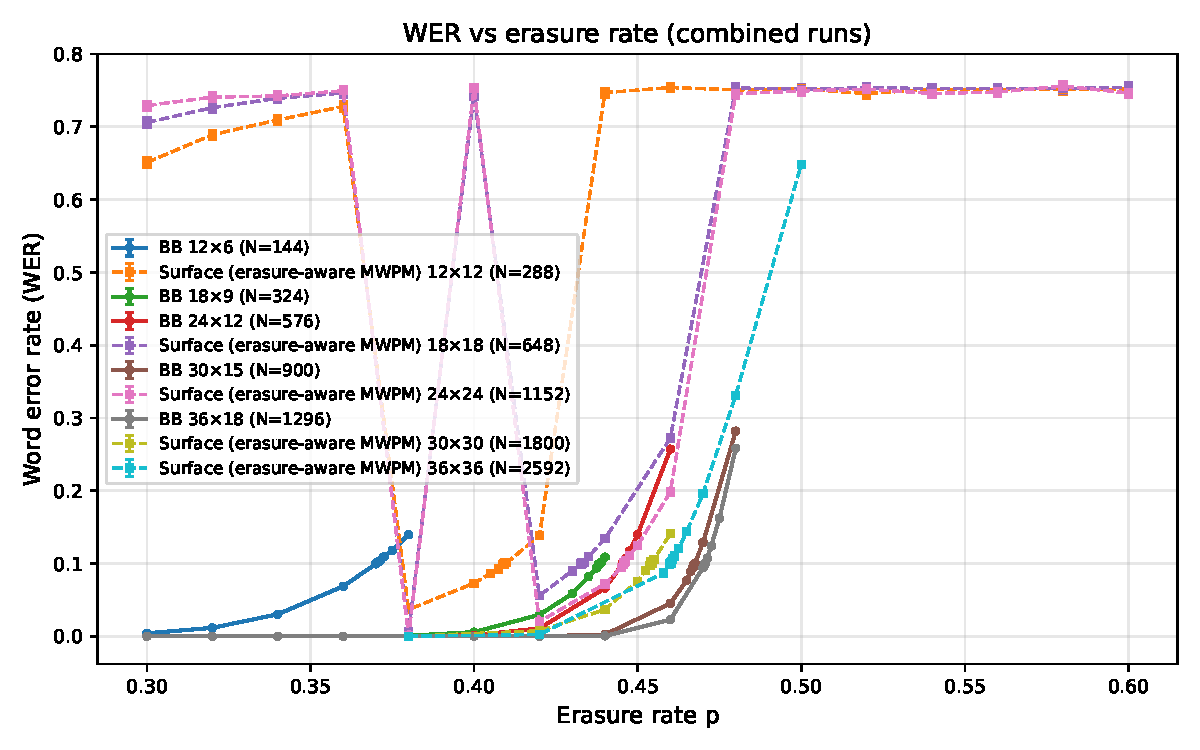
\includegraphics[width=\columnwidth]{plot_all_wer_vs_p.pdf}
\caption{WER vs.\ erasure rate for bivariate bicycle codes (solid lines, $N=144$--$1296$)
and surface code baselines.
Dashed lines: erasure-aware MWPM surface codes ($N=288$--$2592$, $K=2$).
Dotted lines: uninformed MWPM surface codes ($N=288$--$1152$, $K=2$, three sizes).
Error bars show 95\% Wilson confidence intervals.
All BB code curves cross WER = 0.10 at $p^* = 0.37$--$0.47$;
erasure-aware surface codes cross at $p^* = 0.41$--$0.46$.}
\label{fig:wer_curves}
\end{figure}

\subsection{Scaling Behavior and Overhead}

$p^*$ vs.\ $N$ with the FSS asymptote is in Fig.~\ref{fig:pstar_scaling}; $N/K$ runs from
12 (Gross code) to 113 across the five sizes.
Fig.~\ref{fig:overhead_threshold} plots threshold and overhead together: the BB
$[[1296,12]]$ code hits $p^* = 0.471$ at $N/K = 108$, while the erasure-aware surface code
near that threshold needs $N/K = 1296$---12$\times$ worse in this comparison.
That joint advantage is the main practical argument for BB codes here.

\begin{figure}[ht]
\centering
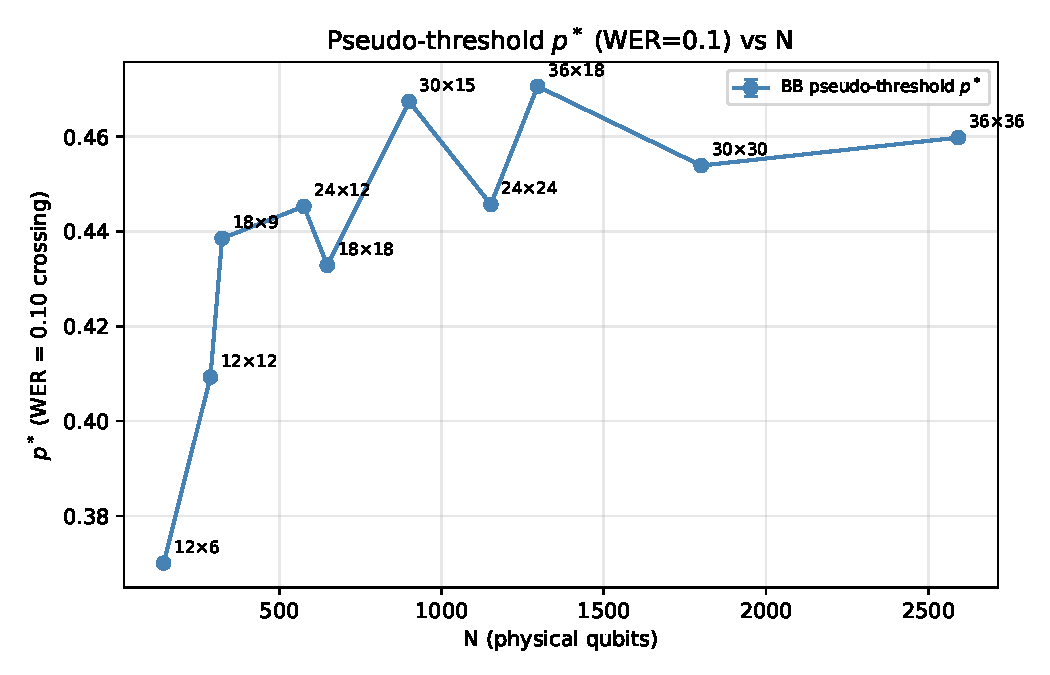
\includegraphics[width=\columnwidth]{plot_all_pstar_vs_N.pdf}
\caption{Pseudo-threshold $p^*$ (WER = 0.10) vs.\ code size $N$ for BB codes.
Error bars show 95\% bootstrap CIs (smaller than markers for large $N$).
The dashed red line and shaded band show the FSS-extrapolated asymptotic threshold
$p^*_\infty = 0.488 \pm 0.001$.}
\label{fig:pstar_scaling}
\end{figure}

\begin{figure}[ht]
\centering
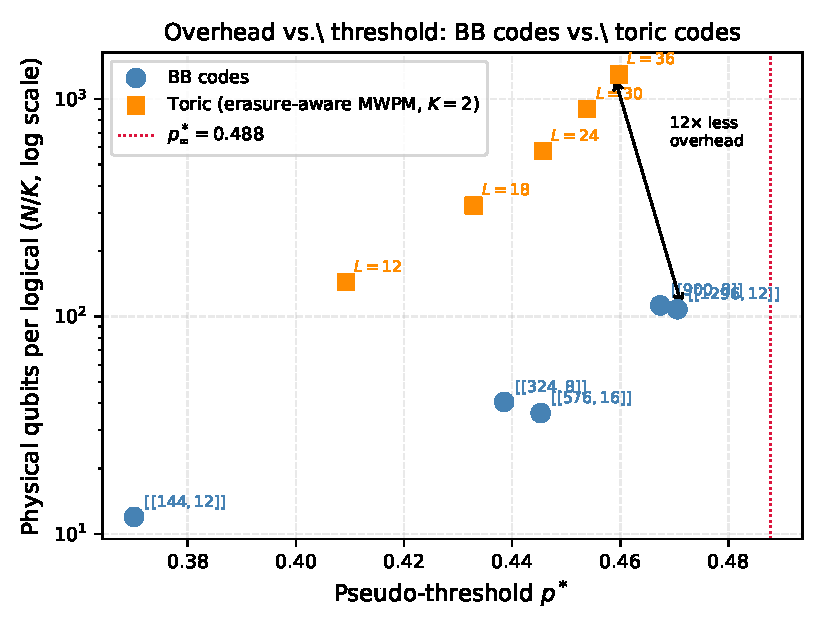
\includegraphics[width=\columnwidth]{plot_overhead_threshold.pdf}
\caption{Overhead ($N/K$, log scale) vs.\ pseudo-threshold $p^*$ for BB codes (circles)
and erasure-aware MWPM surface codes (squares, $K=2$).
A code is better if it appears lower (less overhead) and further right (higher threshold).
BB codes at large $N$ outperform the fixed-$K=2$ surface codes on both axes at these representative sizes.
The annotated arrow highlights the 12$\times$ reduction in normalized overhead between
the $[[1296,12]]$ BB code and the $K=2$ toric code at comparable $p^*$, within this comparison
setting.}
\label{fig:overhead_threshold}
\end{figure}

\subsection{Reproducibility}

Every run is reproducible from recorded data: base seed (12345), per-point worker seeds,
package versions (\texttt{numpy}, \texttt{scipy}, \texttt{bposd}, \texttt{pymatching}), and
platform info in JSON next to the CSV.
Bootstrap CIs use a deterministic seed, so the intervals themselves reproduce.
Few QLDPC simulation papers report seeds or versions; we treat this as part of the
contribution, since reproducing published numbers is otherwise often impossible.

\section{Discussion}

\subsection{Threshold vs.\ Overhead as the Right Metric}

FSS gives an asymptotic erasure threshold $p^*_\infty = 0.488$ for this BB family under
BP-OSD.
The toric code under maximum-likelihood decoding reaches 0.5 \cite{dennis2002topological};
at finite rate $K/N \approx 0.009$--$0.083$ the Shannon limit $1 - K/N$ is much higher, so
the right benchmark is the zero-rate bound $p = 0.5$.
We get \textbf{97.6\% of that} with BP-OSD and no ML decoding---so BP-OSD is effectively
near-optimal for this code on the erasure channel.

Fig.~\ref{fig:frac_capacity} plots $p^*/(1 - K/N)$ vs.\ $N$: it rises from 0.40 at $N=144$
to 0.48 at $N=1296$, trending to 0.488 (97.6\% of the zero-rate limit).
BP-OSD is thus nearly capacity-approaching for large BB codes here.

\begin{figure}[ht]
\centering
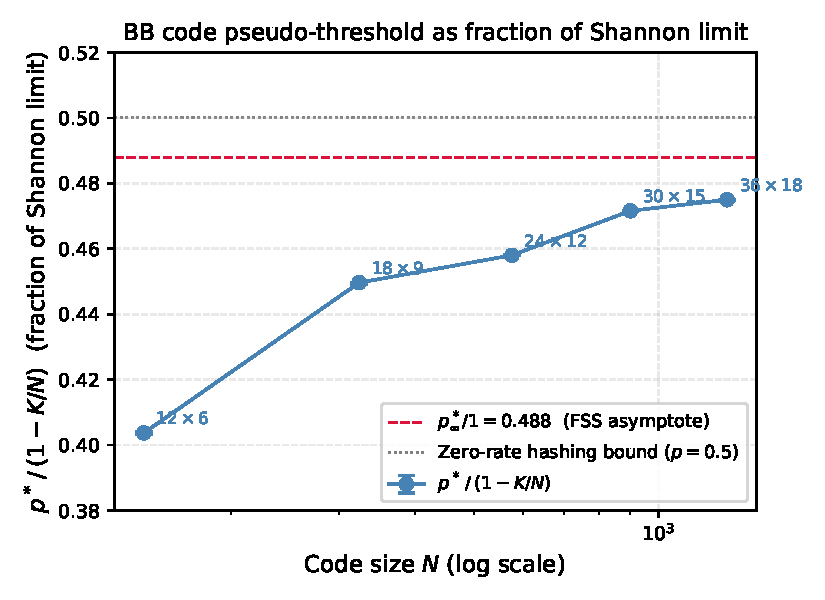
\includegraphics[width=\columnwidth]{plot_fraction_capacity.pdf}
\caption{Pseudo-threshold $p^*$ as a fraction of the Shannon limit $(1 - K/N)$ vs.\ $N$.
Each code's Shannon limit for the erasure channel is $p_{\mathrm{hash}} = 1 - K/N$.
The ratio $p^*/(1-K/N)$ converges to $p^*_\infty = 0.488$ (dashed, asymptotic) as $N\to\infty$,
reaching 97.6\% of the zero-rate limit $p=0.5$ (dotted).
Error bars show 95\% bootstrap CIs propagated through the ratio.}
\label{fig:frac_capacity}
\end{figure}

The threshold edge for BB over erasure-aware surface is real but small
($\Delta p^* \approx 0.01$--$0.03$).
The compelling part is overhead: at comparable $p^*$, BB needs $\sim$12$\times$ fewer
physical qubits per logical qubit (Fig.~\ref{fig:overhead_threshold}).
For constant-rate QLDPC, $K \propto N$ as $N$ grows; for fixed-$K$ surface codes it does
not, so the gap grows in the asymptotic regime.

\subsection{Rate--Threshold Trade-off}

The Gross code $[[144,12,12]]$ has the best rate ($K/N = 0.083$) and $p^* = 0.370$---good
when qubit count matters more than threshold.
Larger codes push $p^*$ up to 0.471 but drop the rate to 0.009.
That trade-off is built into the family and matters for choosing a code on real hardware.

\subsection{Critical Exponent and Universality}\label{sec:critical_exponent}

We get $\nu \approx 1.18$, consistent with a second-order transition.
The surface code maps to the random-bond Ising model (RBIM), which has $\nu = 4/3$
\cite{dennis2002topological, wang2003quantum}---but that mapping assumes ML decoding and a
local Hamiltonian, neither of which holds for BB codes under BP-OSD.
So comparing our $\nu$ to $4/3$ is suggestive, not definitive.

The gap could be finite-size or corrections-to-scaling that our polynomial ansatz misses, or
BB under BP-OSD could sit in a different effective universality class.
Decoder-dependent universality (critical behavior set by the decoder as much as the code) is
plausible for non-local codes with iterative decoding.
Sorting this out would need larger $N$ and a tighter handle on corrections; we leave it
open.
The main results---$p^*_\infty$, overhead, and the fairness correction---do not hinge on
which interpretation is right.

\subsection{Limitations}\label{sec:limitations}

\begin{itemize}
    \item \textbf{Code-capacity channel only}: No circuit-level noise. Circuit-level
          simulations, which include measurement errors and syndrome extraction overhead,
          would more accurately reflect hardware performance and are standard in 2025+
          literature \cite{berthusen2025local}. The code-capacity erasure channel studied
          here is an idealized setting; circuit-level thresholds are typically lower.
    \item \textbf{Fixed decoder}: BP-OSD parameters are fixed at OSD order 10. Adaptive
          tuning or alternative decoders such as localized statistics decoding
          \cite{hillmann2025lsd} or decision-tree decoders \cite{ott2025decision} may
          yield higher thresholds; known limitations of BP for QLDPC codes are discussed
          in iOlius et al.\ \cite{iolius2024bp}.
    \item \textbf{Single polynomial family}: We study one polynomial pair
          ($A = x^3 + y + y^2$, $B = y^3 + x + x^2$). This family was chosen because it
          is the primary BB code in Bravyi et al.\ \cite{bravyi2024high} and has the most
          prior literature, not because it was selected for high threshold.
          Nevertheless, results may not generalize to other BB families; different
          polynomial pairs can yield different distance scaling and threshold behavior.
          Extending to additional families---as partially explored in Rabeti and Mahdavifar
          \cite{rabeti2025bicycle}---would substantially strengthen generality claims
          and is an important direction for future work.
    \item \textbf{Surface code shot count}: Erasure-aware surface code baseline used 50{,}000
          shots per point (versus 200{,}000 for BB codes), giving wider bootstrap CIs on $p^*$.
          The $L=36$ result was confirmed with 200{,}000 shots.
          The larger uncertainty on the surface code side does not affect qualitative
          conclusions: the threshold differences between BB and surface codes exceed the CI
          overlap even under the asymmetric shot counts.
    \item \textbf{Architectural comparison}: The overhead comparison between BB and surface
          codes is not fully architecture-neutral. Surface codes are constrained to $K=2$ by
          their local planar structure; BB codes are non-local. The $12\times$ overhead
          figure should be interpreted as a difference in code efficiency within this
          comparison setting, not as a universal hardware advantage.
\end{itemize}

\section{Conclusion}

We simulated bivariate bicycle codes on the quantum erasure channel and tackled two
methodological issues that distort many QLDPC comparisons: decoder-baseline fairness and
the confusion of pseudo-thresholds with asymptotic thresholds.
Without erasure information, standard MWPM on the surface code matches random guessing in
our regime---so fair code comparisons need erasure-aware MWPM, and the old baseline
systematically misleads.
On that fair baseline, BB pseudo-thresholds run from $p^* = 0.370$ to $0.471$ for
$N = 144$--$1296$ (95\% bootstrap CIs $\lesssim 0.001$), and FSS extrapolates
$p^*_\infty \approx 0.488$ ($\pm 0.001$ stat, $\lesssim 0.005$ sys) with $\nu \approx 1.18$.
BB has a small threshold edge and a 12$\times$ lower normalized overhead than surface
codes in this setting.

The practical message: BB codes compete on the erasure channel mainly through qubit
efficiency, not raw threshold.
We also provide a reproducible pipeline (seeds, versions, metadata) so that future work on
decoders or code families can build on numbers that actually replicate.

\section*{Acknowledgments}

We thank the QLDPC community for the code constructions that made this work possible, and the
developers of \texttt{bposd}, \texttt{ldpc}, and \texttt{pymatching} for the tools we used.

\begin{thebibliography}{99}

\bibitem{bravyi2024high}
Bravyi, S., Cross, A. W., Gambetta, J. M., Maslov, D., Rall, P., \& Yoder, T. J. (2024).
High-threshold and low-overhead fault-tolerant quantum memory.
\textit{Nature}, 627, 778--782.
\url{https://arxiv.org/abs/2308.07915}

\bibitem{nielsen2010quantum}
Nielsen, M. A., \& Chuang, I. L. (2010).
\textit{Quantum Computation and Quantum Information}.
Cambridge University Press.

\bibitem{gottesman1997stabilizer}
Gottesman, D. (1997).
Stabilizer codes and quantum error correction.
PhD thesis, Caltech.
\url{https://arxiv.org/abs/quant-ph/9705052}

\bibitem{tillich2014quantum}
Tillich, J., \& Z\'emor, G. (2014).
Quantum LDPC codes with positive rate and minimum distance proportional to the square root of the blocklength.
\textit{IEEE Transactions on Information Theory}, 60(2), 1193--1202.
\url{https://arxiv.org/abs/1202.0928}

\bibitem{kovalev2013improved}
Kovalev, A. A., \& Pryadko, L. P. (2013).
Improved quantum hypergraph-product LDPC codes.
\textit{IEEE Transactions on Information Theory}, 59(12), 8318--8330.
\url{https://arxiv.org/abs/1302.0318}

\bibitem{dennis2002topological}
Dennis, E., Kitaev, A., Landahl, A., \& Preskill, J. (2002).
Topological quantum memory.
\textit{Journal of Mathematical Physics}, 43(9), 4452--4505.
\url{https://arxiv.org/abs/quant-ph/0110143}

\bibitem{fowler2012surface}
Fowler, A. G., Mariantoni, M., Martinis, J. M., \& Cleland, A. N. (2012).
Surface codes: Towards practical large-scale quantum computation.
\textit{Physical Review A}, 86(3), 032324.
\url{https://arxiv.org/abs/1208.0928}

\bibitem{grassl2004codes}
Grassl, M., R\"otteler, M., \& Beth, T. (2004).
On optimal quantum codes.
\textit{International Journal of Quantum Information}, 2(1), 55--64.
\url{https://arxiv.org/abs/quant-ph/0312164}

\bibitem{roffe2020decoding}
Roffe, J., White, D. R., Burton, S., \& Campbell, E. (2020).
Decoding across the quantum low-density parity-check code landscape.
\textit{Physical Review Research}, 2(4), 043423.
\url{https://arxiv.org/abs/2005.07016}

\bibitem{pymatching}
Higgott, O., \& Gidney, C. (2022).
PyMatching: A Python package for decoding quantum codes with minimum-weight perfect matching.
\url{https://github.com/oscarhiggott/PyMatching}

\bibitem{edmonds1965paths}
Edmonds, J. (1965).
Paths, trees, and flowers.
\textit{Canadian Journal of Mathematics}, 17, 449--467.

\bibitem{kolmogorov2009blossom}
Kolmogorov, V. (2009).
Blossom V: A new implementation of a minimum cost perfect matching algorithm.
\textit{Mathematical Programming Computation}, 1(1), 43--67.

\bibitem{chung2001design}
Chung, S. Y., Forney, G. D., Richardson, T. J., \& Urbanke, R. (2001).
On the design of low-density parity-check codes within 0.0045 dB of the Shannon limit.
\textit{IEEE Communications Letters}, 5(2), 58--60.

\bibitem{richardson2008modern}
Richardson, T., \& Urbanke, R. (2008).
\textit{Modern Coding Theory}.
Cambridge University Press.

\bibitem{panteleev2022asymptotically}
Panteleev, P., \& Kalachev, G. (2022).
Asymptotically good quantum and locally testable classical LDPC codes.
\textit{Proceedings of the 54th Annual ACM SIGACT Symposium on Theory of Computing}, 375--388.
\url{https://arxiv.org/abs/2111.03654}

\bibitem{breuckmann2021quantum}
Breuckmann, N. P., \& Eberhardt, J. N. (2021).
Quantum low-density parity-check codes.
\textit{PRX Quantum}, 2(4), 040101.
\url{https://arxiv.org/abs/2002.11169}

\bibitem{leverrier2015quantum}
Leverrier, A., Tillich, J. P., \& Z\'emor, G. (2015).
Quantum expander codes.
\textit{Proceedings of the 56th Annual IEEE Symposium on Foundations of Computer Science}, 810--824.
\url{https://arxiv.org/abs/1504.00815}

\bibitem{wang2003quantum}
Wang, C., Harrington, J., \& Preskill, J. (2003).
Confinement-Higgs transition in a disordered gauge theory and the accuracy threshold for quantum memory.
\textit{Annals of Physics}, 303(1), 31--58.
\url{https://arxiv.org/abs/quant-ph/0207088}

\bibitem{berthusen2025local}
Berthusen, N., Pham, T., Gottesman, D., \& Hangleiter, D. (2025).
Toward a 2D local implementation of quantum LDPC codes.
\textit{PRX Quantum}, 6, 010306.
\url{https://link.aps.org/pdf/10.1103/PRXQuantum.6.010306}

\bibitem{pecorari2025qldpc}
Pecorari, L., \& Pupillo, G. (2025).
Quantum LDPC codes for erasure-biased atomic quantum processors.
\textit{Physical Review A}.
\url{https://arxiv.org/abs/2502.20189}

\bibitem{bhave2026bibi}
Bhave, A. S., Hann, C. T., \& Aaronson, S. (2026).
BiBiEQ: Bivariate bicycle codes on erasure qubits.
\textit{arXiv preprint arXiv:2602.07578}.
\url{https://arxiv.org/abs/2602.07578}

\bibitem{hillmann2025lsd}
Hillmann, T., Berent, L., Townsend-Teague, A., Eisert, J., Roffe, J., \& Strikis, A. (2025).
Localized statistics decoding: A parallel decoding algorithm for quantum low-density
parity-check codes.
\textit{Nature Communications}.
\url{https://arxiv.org/abs/2406.18655}

\bibitem{liang2025bposd}
Liang, J., et al. (2025).
A low-complexity BP-OSD algorithm for quantum LDPC codes.
\textit{The European Physical Journal Special Topics}.

\bibitem{ott2025decision}
Ott, K. R., et al. (2025).
Decision-tree decoders for quantum LDPC codes.
\textit{arXiv preprint arXiv:2502.16408}.
\url{https://arxiv.org/abs/2502.16408}

\bibitem{yin2024symmetry}
Yin, K., et al. (2024).
Symmetry-breaking decoding for quantum LDPC codes.
\textit{arXiv preprint arXiv:2412.02885}.
\url{https://arxiv.org/abs/2412.02885}

\bibitem{gong2024bpdecoding}
Gong, Z., et al. (2024).
Low-latency belief propagation decoding for quantum LDPC codes.
\textit{arXiv preprint arXiv:2403.18901}.
\url{https://arxiv.org/abs/2403.18901}

\bibitem{rabeti2025bicycle}
Rabeti, M., \& Mahdavifar, H. (2025).
Constructions and analysis of bivariate bicycle codes.
\textit{arXiv preprint arXiv:2511.02951}.
\url{https://arxiv.org/abs/2511.02951}

\bibitem{iolius2024bp}
iOlius, A., et al. (2024).
Limitations of belief propagation for QLDPC codes.
\textit{arXiv preprint arXiv:2409.01440}.
\url{https://arxiv.org/abs/2409.01440}

\end{thebibliography}

\end{document}
